\section{Fundamentals}
Gravitational Waves (GW) are oscillations in spacetime, similar to electromagnetic
waves. We can start with the Einstein equation:

\begin{equation}
    G_{\mu\nu}= \frac{8\pi G}{c^4} T_{\mu\nu}.
\end{equation}

Since GW (mostly) propagate in the vacuum and we assume a small amplitude $|\delta g_{\mu\nu}| \ll 1$, we arrive at the following differential equation.

\begin{equation}
    T_{\mu\nu} = 0
\end{equation}
\begin{equation}
    \Rightarrow G_{\mu\nu} = 0
\end{equation}


We assume that the metric only has small linear perturbations. 
\begin{equation}
    g_{\mu \nu}(t, \vec{x}) = \bar{g}_{\mu \nu}(t) + \delta g_{\mu \nu}(t, \bar{x})
\end{equation}
\begin{equation}
   = \eta_{\mu \nu} + h_{\mu \nu}
\end{equation}
\begin{equation}
    |h_{\mu \nu}| << 1
\end{equation}
Here $\eta_{ \mu \nu}$ the Minkowski metric for flat spacetime.

We can solve the differential equation with the trace reverse tensor.

\begin{equation}
    \bar{h}_{\mu\nu} = h_{\mu\nu}-\frac{1}{2} \eta_{\mu\nu}h
\end{equation}

Here, $h$ is the trace of $h_{\mu\nu}$.

For a plane wave moving in the z-direction with plus polarization (explain), we would 
have the following perturbation.
\begin{equation}
    h(z, t) = h_+ 
    \begin{pmatrix}
        1 & 0 & 0 \\ 0 & -1 & 0 \\ 0 & 0 & 0
    \end{pmatrix}
    e^{i(k z-\omega t)}
\end{equation}
For a length of $L_0$ along the x-axis, it would oscillate in size in the
following way:
\begin{equation}
    L(t) = L_0 + \frac{h_+ L_0}{2} cos(\omega t).
\end{equation}

\section{Sources}
Gravitational Waves can be created by different sources. These can be
merging binaries, bursts (e.g. from core-collapse supernovae), continuous waves 
(e.g. from pulsars) and a stochastic background (see below).

\subsection{Binary Black Hole Mergers}
In this work, we focus on binary black holes. Since most resolved events from LIGO/Virgo are binary black holes. In a recent analysis of the Gravitational Wave Transient Catalogue 3 (GWTC-3), they considered 69 events with a false alarm rate of less than $\frac{1}{4}$ per year. Out of this sample, 63 came from binary black holes, 2 from binary neutron stars and 2 from neutron star-black hole mergers.

If we consider the energy density parameter of the stochastic GW background, we see that binary black holes dominate at lower frequencies up to around 600 Hz, see 

\begin{figure}[h]
    \centering
    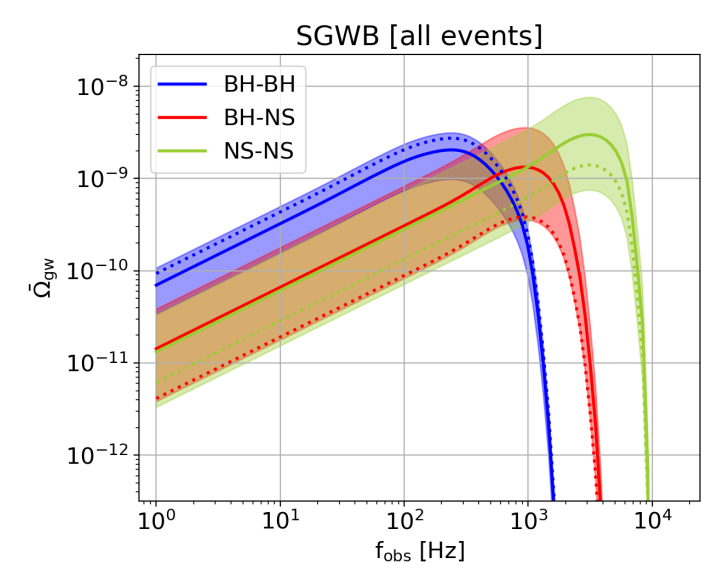
\includegraphics[width=0.7\linewidth]{Images/Capurri_GW_Background_monopole_sources.png}
    \caption{The GW energy density parameter as a function of frequency from 1 to 10,000 Hz. This shows the different contributions from BH-BH, NS-NS and BH-NS events. The Figure is taken from Ref. \cite{capurri_intensity_2021}.}
    \label{BG_sources}
\end{figure} 

\begin{figure}[h]
    \centering
    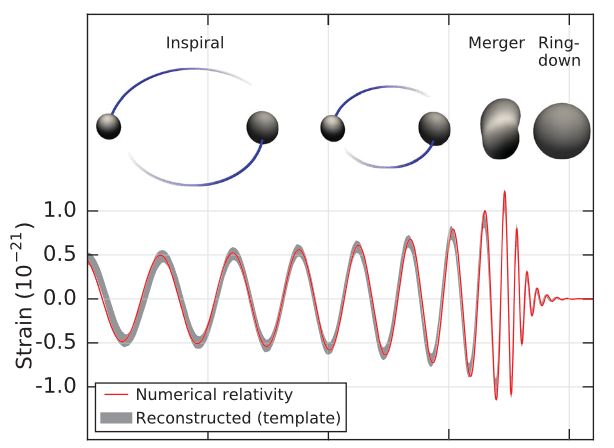
\includegraphics[width=0.7\linewidth]{Images/waveform-abbott.PNG}
    \caption{The different stages of a BBH merger with the corresponding waveform, here an illustrative estimate of GW150914. The Figure is taken from Ref.\ \cite{abbott_observation_2016}.}
    \label{GW_waveform}
\end{figure} 

From the waveform, we can extrapolate black hole properties, like the chirp mass and the spin. 

\begin{equation}
    \mathcal{M}_c = \frac{(m_1m_2)^{3/5}}{(m_1+m_2)^{1/5}}
\end{equation}

The frequency is determined by the total mass. 
The waveform can be decomposed into harmonic, where the quadrupole ($(\ell, m)=(2,2)$) is naturally the dominant one. 
(insert from Bonn lectures?)

\section{Stochastic Background}
For the stochastic background, we need the correlation between two detector
outputs \cite{christensen_stochastic_2019}.
\begin{equation}
    \langle s_1 (t) s_2(t)\rangle \, = \, \langle(n_1(t) + h(t))(n_2(t) + h(t))\rangle
\end{equation}
\begin{equation}
    = \, \langle n_1(t) n_2(t)\rangle + \langle n_1(t)h(t)\rangle + \langle h(t)n_2(t)\rangle  + \langle h(t)h(t)\rangle  
\end{equation}
\begin{equation}
    \approx \, \langle h(t)h(t)\rangle 
\end{equation}
From there we can compute the root mean square of the strain.
\begin{equation}
    h_{rms}^2 = \langle \sum_{i,j} h_{ij} h_{ij}\rangle 
\end{equation}
\begin{equation}
    = \int_0^\infty df \, S_h (f)
\end{equation}
Here $S_h$ is the spectral density, from which we can derive the GW energy
density.
\begin{equation}
    \rho_{GW} = \int_0^\infty df \, S_h(f) \frac{\pi c^2 f^2}{8G}
\end{equation} 
\subsection{Astrophysical}


Anisotropy limits from LIGO:
(check for more current)
The LIGO anisotropy limit for the first observing run O1 published in 2017
was 
\begin{equation}
    \Omega_{2/3} = (4.4 \pm 6.4) \cdot 10^{-8} .
\end{equation}

This is compatible with zero, but an anisotropic background would indicate
a more interesting cosmology, which is why it would be important to disentangle
any anisotropic that could be observed.

The astrophysical GW background was detected for the first time this year (2023) using the pulsar time array NANOGrav \cite{agazie_nanograv_2023}. Pulsar time arrays use the fact that pulsars are very accurate clocks. They are rotating neutron stars that have a strong magnetic field and thus emit radio waves in very regular intervals. Since they are so stable, we can use these signals as accurate clocks. If there are any changes in the time of arrival of multiple pulsars, this could indicate a gravitational wave background. 
The NANOGrav experiment used a frequency range of $10^{8.75} - 10^{7.5}$ Hz. They assumed a GW energy density parameter proportional to $f^{-2/3}$, which is the case in the inspiral phase of binary black holes. \cite{phinney_practical_2001}
Using this, they find an integrated energy density $\Omega_{GW} = 9.3^{+5.8}_{-4.0}\cdot 10^{-9}$.

\subsubsection{Dipole}
The cosmological principle says, that the universe is isotropic and homogeneous on large scales. Gravitational Waves are one mode of testing this further. If we find anisotropies in the GW background, other than the kinematic dipole and shot noise, this would be evidence against the principle.
The kinematic dipole arises from the observer motion with respect to the large-scale structure rest frame. More GW events should be detected in the direction in which we move, and fewer in the opposite direction. Shot noise comes from stochastic fluctuations in the background, which follow a Poisson distribution.

The GW density contrast can be written with an integration over the window function, which weights the contributions in the redshift domain.

\begin{equation}
    \delta(f_0, \hat{n}) = \frac{\Omega(f_0, \hat{n})-\overline{\Omega}(f_0)}{\overline{\Omega}(f_0)}
\end{equation}
\begin{equation}
    = \int dz \; W(f_0, z) \; \Delta(f_0, \hat{n}, z)
\end{equation}

...
\subsection{Cosmological}
The major contributions to the cosmological GW background are primordial
black holes and gravitational waves from phase transitions and inflation.
Schulze et al. \cite{schulze_gw_class_2023} computed the angular power spectrum 
of this background using a modified version of CLASS\cite{blas_cosmic_2011}.
\subsubsection{Primordial Black Holes}
...
\subsubsection{Inflation}

A period of inflation in the early universe solves two important cosmological problems, namely the flatness and the horizon problem. The flatness problem arises when we assume radiation domination followed by matter domination which is followed by $\Lambda$ (the cosmological constant) domination. The spatial curvature density parameter is measured to be very low. 
\begin{equation}
    |\Omega_k| = \frac{\rho_k^{\rm{eff}}}{\rho_{crit}} < 10^{-2}
\end{equation} 
On the other hand, the radiation energy density parameter is of an even lower order.
\begin{equation}
    |\Omega_r| = \frac{\rho_r}{\rho_{crit}} \in \mathcal{O}(10^{-4}) 
\end{equation}

Now the effective curvature energy density $\rho_{k}^{\rm{eff}}$ scales like $a^{-2}$, while the radiation energy density $\rho_{r}$ scales like $a^{-4}$, with the scale factor a.
At the Planck time $t_P = \sqrt{\frac{\hbar G}{c^5}}$ the ratio between them was many orders of magnitudes lower than 1.
\begin{equation}
    \frac{|\rho_k^{\rm{eff}}(t_P)|}{\rho_r(t_P)} \approx 10^{-62}
\end{equation}

This seems unlikely since we would expect roughly the same order of magnitude for all the energy density parameters $\rho_m, \rho_r, \rho_\Lambda, \rm{ and } \, \rho_k^{eff}$. Random initial conditions would lead us to the same order of magnitude of these parameters.
We also know how $\Omega_k$ scales with the scale factor.
\begin{equation}
    \Omega_k = - \frac{k}{(aH)^2}= -\frac{k}{\dot{a}^2}
\end{equation}

In the case of an inflationary GW background, the tensor power spectrum $P_T(k)$ creates the GW. This is linearly related to the average GW energy density parameter (or monopole) \cite{schulze_gw_class_2023}.

\begin{equation}
    \bar{\Omega}_{GW} = \frac{1}{12 H_0^2 a_0^2} \frac{\eta_{eq}^2}{2\eta_0^4} P_T(k)
\end{equation}

The GW created through large-scale perturbations during inflation are relevant for wavenumbers $k=10^{-5} Mpc^{-1} -1 Mpc^{-1}$, which corresponds to millihertz up to the Hertz range, going through both the sensitivity range of ground-based detectors, like ET \cite{alonso_noise_2020}, and space-based detectors like LISA \cite{robson_construction_2019}.

\subsubsection{Phase Transitions}

Bubbles of a phase can form in a universe which is in an older phase. In there, magnetohydrodynamic (MHD) turbulence can also produce GW.

...

\subsection{Number Density Distribution}

The {\tt Multi\_CLASS} code uses the number density of detectable GW per redshift per solid angle element from \cite{scelfo_gwtimeslss_2018}:

\begin{equation}
    \frac{d^2N_{GW}}{dzd\Omega} = T_{obs}\frac{c\chi^2(z)}{(1+z)H(z)}R_{tot}(z)F_{GW}^{detectable}(z).
\end{equation}

$T_{obs}$ is the total observational time, $\chi(z)$ is the comoving distance, $H(z)$ is the Hubble rate, $R_{tot}(z)$ is the total comoving merger rate and $F_{GW}^{detectable}(z)$ the fraction of detectable events. For the merger rate, they include primordial black holes and binary BH (abbr) in their calculation.
The authors choose the common SNR threshold $\langle \rho^2 \rangle =8$.
\begin{equation}
    \langle \rho^2 \rangle = \frac{1}{5}\int_{f_{min}}^{f_{max}} df \frac{h_c^2(f)}{f^2 S_n(f)}
\end{equation}

For the Einstein Telescope (ET), they find that $F_{GW}^{detectable} \approx 1$ even for redshifts above 5, which have a small effect on the detection overall.

\subsection{Projection Effects}

\textit{change style,}
\textit{explain physics-> papers Yoo, Bonvin}

For the intrinsic anisotropies, there are different contributions to the source functions $\Delta_l^{AGWB}$. The different pertinent effects are density fluctuations, redshift space distortions, the Doppler effect and relativistic corrections or gravitational potential terms. \cite{di_dio_classgal_2013}.

We write each random field as a product of the primordial curvature perturbation and a transfer function. In \cite{dallarmi_dipole_2022}, they compute the different source terms using the {\tt CLASSgal} framework. The implementation in {\tt CLASS} follows the same framework, since {\tt CLASSgal} has been merged into the standard public code.

\begin{equation}
    X(\eta, \vec{k}) = T_X(\eta, \vec{k})\zeta(\vec{k})
\end{equation}

The two-point correlation function of the curvature perturbation has the following form.

\begin{equation}
    \langle \zeta(\vec{k})\zeta*(\vec{k}')\rangle = (2\pi)^3 \delta(\vec{k}-\vec{k}')\frac{2\pi^2}{k^3}P(k)
\end{equation}

There is one density source term, dependent on the transfer functions of matter density fluctuations $T_{\delta m}$ and of the velocity divergence of matter $T_{\theta m}$. Here, $\bar{\chi}$ is a shifted conformal time variable.

\begin{equation}
    \bar{\chi} = \eta_0 - \eta 
\end{equation}


\begin{equation}
    \Delta_\ell^{den}=\int_0^{\eta_0} d\eta W \left(b T_{\delta m} +3 \frac{aH}{k^2} T_{\theta_m}\right)j_l(k \bar{\chi})
\end{equation}

Here, $j_l(k \bar{\chi})$ is the spherical bessel function and we integrate over conformal time using the window function, like in the following source contributions.

The Doppler terms also depend on the velocity divergence of matter since the velocity determines the Doppler effect.

\begin{equation}
    \Delta_\ell^{D1}=\int_0^{\eta_0} d\eta W \frac{T_{\theta_m}}{k} \left(-b_e + \frac{H'}{aH^2}+3\right)\frac{d}{d(k\bar{\chi})} j_l(k \bar{\chi})
\end{equation}

\begin{equation}
    \Delta_\ell^{D2}=\int_0^{\eta_0} d\eta W T_{\theta_m}(b_e-3) \frac{aH}{k^2} j_l(k \bar{\chi})
\end{equation}

The term for the redshift space distortions was derived by \cite{kaiser} and depends on the second derivative of the bessel function.

\begin{equation}
    \Delta_\ell^{RSD}=\int_0^{\eta_0} d\eta W T_{\theta_m} \frac{1}{aH}\frac{d^2}{d(k\bar{\chi})^2} j_l(k \bar{\chi})
\end{equation}

There are five relativistic corrections, which can also be called gravitational potential terms since the redshift space distortions are also relativistic. In the GW case, two of these terms vanish (\cite{dallarmi_dipole_2022}), while the other three are non-zero.

\begin{equation}
    \Delta_\ell^{G1}=\int_0^{\eta_0} d\eta W T_\Psi \left(4-b_e+\frac{H}{aH^2}\right) j_l(k \bar{\chi})
\end{equation}

\begin{equation}
    \Delta_\ell^{G3}=\int_0^{\eta_0} d\eta W T_{\Phi'} \frac{1}{aH} j_l(k \bar{\chi})
\end{equation}

\begin{equation}
    \Delta_\ell^{G5}=\int_0^{\eta_0} d\eta W \left(-b_e + \frac{H'}{aH^2} +3\right) \int_0^{\tilde{\eta}} d\tilde{\eta} j_l(k \bar{\chi}) \left( T_{\Phi'}(\tilde{\eta})T_{\Psi'}(\tilde{\eta})-\frac{1}{2}T'_{h, ij}(\tilde{\eta})n^i n^j \right)
\end{equation}

In the last equation $n^i$ are the components of the line of sight vector.

\begin{equation}
    \label{window_fct_def}
        \delta_{AGWB}(f_0, \hat{n})=\int dz \tilde{W}(f_0, z)\Delta_{AGWB}(f_0, \hat{n}, z)
    \end{equation}

\begin{equation}
    \begin{split}
        = \int d\bar{\chi} \tilde{W} [b(\delta_m - 3\mathcal{H}V)+(3-b_e)\mathcal{H}V+
        \Psi(3-b_e+\frac{\mathcal{H'}}{\mathcal{H}^2})+2I(b_e
        -\frac{\mathcal{H'}}{\mathcal{H}^2}-2) \\
        +(\delta a_0+\Psi_0 - v_{\parallel 0})(b_e
        -\frac{\mathcal{H'}}{\mathcal{H}^2}-2)-v_\parallel (-b_e
        +\frac{\mathcal{H'}}{\mathcal{H}^2}+2) \\
        +\frac{1}{\mathcal{H}}\Phi' 
        -\frac{1}{\mathcal{H}}\partial_\parallel v_\parallel 
        - \frac{1}{2\mathcal{H}}h_{ij}'^{TT} n^i n^j]
    \end{split}
    \end{equation}
    Here the following notation is used:
    \begin{equation}
            v_\parallel = \hat{n} \vec{v} 
    \end{equation}
    \begin{equation}
            \partial{\parallel} = \hat{n} \vec{\nabla} 
    \end{equation}
    \begin{equation}
            I(\bar{\chi}) = -\frac{1}{2} \int_0^{\bar{\chi}} d\tilde{\chi} 
            (\Psi' + \Phi ' -\frac{1}{2}h_{ij}')(\tilde{\chi} )
    \end{equation}
    \begin{equation}
            \vec{v} = \vec{\nabla} V 
    \end{equation}


